% В этом файле следует писать текст работы, разбивая его на
% разделы (section), подразделы (subsection) и, если нужно,
% главы (chapter).

% Предварительно следует указать необходимую информацию
% в файле SETUP.tex

%% В этот файл не предполагается вносить изменения

% В этом файле следует указать информацию о себе
% и выполняемой работе.

\documentclass [fontsize=14pt, paper=a4, pagesize, DIV=calc]%
{scrreprt}
% ВНИМАНИЕ! Для использования глав поменять
% scrartcl на scrreprt

% Здесь ничего не менять
\usepackage [T2A] {fontenc}   % Кириллица в PDF файле
\usepackage [utf8] {inputenc} % Кодировка текста: utf-8
\usepackage [russian] {babel} % Переносы, лигатуры

%%%%%%%%%%%%%%%%%%%%%%%%%%%%%%%%%%%%%%%%%%%%%%%%%%%%%%%%%%%%%%%%%%%%%%%%
% Создание макроса управления элементами, специфичными
% для вида работы (курс., бак., маг.)
% Здесь ничего не менять:
\usepackage{ifthen}
\newcounter{worktype}
\newcommand{\typeOfWork}[1]
{
	\setcounter{worktype}{#1}
}

% ВНИМАНИЕ!
% Укажите тип работы: 0 - курсовая, 1 - бак., 2 - маг.,
% 3 - бакалаврская с главами.
\typeOfWork{2}
% Считается, что курсовая и бак. бьются на разделы (section) и
% подразделы (subsection), а маг. — на главы (chapter), разделы и
%  подразделы. Если хочется,
% чтобы бак. была с главами (например, если она большая),
% надо выбрать опцию 3.

% Если при выборе 2 или 3 вы забудете поменять класс
% документа на scrreprt (см. выше, в самом начале),
% то получите ошибку:
% ./aux/appearance.tex:52: Package scrbase Error: unknown option ` chapterprefix=

%%%%%%%%%%%%%%%%%%%%%%%%%%%%%%%%%%%%%%%%%%%%%%%%%%%%%%%%%%%%%%%%%%%%%%%%
% Информация об авторе и работе для титульной страницы

\usepackage {titling}

% Имя автора в именительном падеже (для маг.)
\newcommand {\me}{%
А.\,С.~Коваленко%
}

% Имя автора в родительном падеже (для курсовой и бак.)
\newcommand {\byme}{%
А.\,С.~Коваленко%
}

% Любимый научный руководитель
\newcommand{\supervisor}%
{учёная степень, учёное звание /  должность И. О. Фамилия}

% идентифицируем пол (только для курсовой и бак.)
\newcommand{\bystudent}{
Студента %Студентки % Для курсовой: с большой буквы
}

% Год публикации
\date{2020}

% Название работы
\title{Обучение шумоподавляющей нейронной сети без использования чистых данных}

% Кафедра
%
\newboolean{needchair}
\setboolean{needchair}{false} % на ФИИТ не пишется (false), на ПМИ есть (true)

\newcommand {\thechair} {%
Кафедра компьютерного и аналогового моделирования светлого будущего%
}

\newcommand {\direction} {%
Направление подготовки\\
Фундаментальная информатика и информационные технологии%
}% Прикладная математика и информатика

%%%%%%%%%%%%%%%%%%%%%%%%%%%%%%%%%%%%%%%%%%%%%%%%%%%%%%%%%%%%%%%%%%%%%%%%
% Другие настраиваемые элементы текста

% Листинги с исходным кодом программ: укажите язык программирования
\usepackage{listings}
\lstset{
    language=[ISO]C++,%  Язык указать здесь
    basicstyle=\small\ttfamily,
    breaklines=true,%
    showstringspaces=false%
    inputencoding=utf8x%
}
% полный список языков, поддерживаемых данным пакетом, есть,
% например, здесь (стр. 13):
% ftp://ftp.tex.ac.uk/tex-archive/macros/latex/contrib/listings/listings.pdf

% Нумерация списков: можно при необходимести
% изменять вид нумерации (например, добавлять правую скобку).
% По умолчанию буду списки вида:
% 1.
% 2.
% Изменять вид нумерации можно в начале нумерации:
% \begin{enumerate}[1)] (В квадратных скобках указан желаемый вид)
\usepackage[shortlabels]{enumitem}
                    \setlist[enumerate, 1]{1.}

% Гиперссылки: настройте внешний вид ссылок
\usepackage%
[pdftex,unicode,pdfborder={0 0 0},draft=false,%backref=page,
    hidelinks, % убрать, если хочется видеть ссылки: это
               % удобно в PDF файле, но не должно появиться на печати
    bookmarks=true,bookmarksnumbered=false,bookmarksopen=false]%
{hyperref}


\usepackage {amsmath}      % Больше математики
\usepackage {amssymb}
\usepackage {textcase}     % Преобразование к верхнему регистру
\usepackage {indentfirst}  % Красная строка первого абзаца в разделе

\usepackage {fancyvrb}     % Листинги: определяем своё окружение Verb
\DefineVerbatimEnvironment% с уменьшенным шрифтом
	{Verb}{Verbatim}
	{fontsize=\small}

% Вставка рисунков
\usepackage {graphicx}

% Общее оформление
% ----------------------------------------------------------------
% Настройка внешнего вида

%%% Шрифты

% если закомментировать всё — консервативная гарнитура Computer Modern
\usepackage{paratype} % профессиональные свободные шрифты
%\usepackage {droid}  % неплохие свободные шрифты от Google
%\usepackage{mathptmx}
%\usepackage {mmasym}
%\usepackage {psfonts}
%\usepackage{lmodern}
%var1: lh additions for bold concrete fonts
%\usepackage{lh-t2axccr}
%var2: the package below could be covered with fd-files
%\usepackage{lh-t2accr}
%\usepackage {pscyr}

% Геометрия текста

\usepackage{setspace}       % Межстрочный интервал
\onehalfspacing

\newlength\MyIndent
\setlength\MyIndent{1.25cm}
\setlength{\parindent}{\MyIndent} % Абзацный отступ
\frenchspacing            % Отключение лишних отступов после точек
\KOMAoptions{%
    DIV=calc,         % Пересчёт геометрии
    numbers=endperiod % точки после номеров разделов
}

                            % Консервативный вариант:
%\usepackage                % ручное задание геометрии
%[%                         % (не рекомендуется в проф. типографии)
%  margin = 2.5cm,
  %includefoot,
  %footskip = 1cm
%] %
%  {geometry}

%%% Заголовки

\ifthenelse{\equal{\theworktype}{2}}{%
\KOMAoptions{%
    numbers=endperiod,% точки после номеров разделов
    headings=normal,   % размеры заголовков поменьше стандартных
    chapterprefix=true,% Печатать слово Глава в магистерской
    appendixprefix=true% Печатать слово Приложение
}
}

% шрифт для оформления глав и названия содержания
\newcommand{\SuperFont}{\Large\sffamily\bfseries}

% Заголовок главы
\ifthenelse{\value{worktype} > 1}{%
\renewcommand{\SuperFont}{\Large\normalfont\sffamily}
\newcommand{\CentSuperFont}{\centering\SuperFont}
\usepackage{fncychap}
\ChNameVar{\SuperFont}
\ChNumVar{\CentSuperFont}
\ChTitleVar{\CentSuperFont}
\ChNameUpperCase
\ChTitleUpperCase
}

% Заголовок (под)раздела с абзацного отступа
\addtokomafont{sectioning}{\hspace{\MyIndent}}

\renewcommand*{\captionformat}{~---~}
\renewcommand*{\figureformat}{Рисунок~\thefigure}

% Плавающие листинги
\usepackage{float}
\floatstyle{ruled}
\floatname{ListingEnv}{Листинг}
\newfloat{ListingEnv}{htbp}{lol}[section]

% точка после номера листинга
\makeatletter
\renewcommand\floatc@ruled[2]{{\@fs@cfont #1.} #2\par}
\makeatother


%%% Оглавление
\usepackage{tocloft}

% шрифт и положение заголовка
\ifthenelse{\value{worktype} > 1}{%
\renewcommand{\cfttoctitlefont}{\hfil\SuperFont\MakeUppercase}
}{
\renewcommand{\cfttoctitlefont}{\hfil\SuperFont}
}

% слово Глава
\usepackage{calc}
\ifthenelse{\value{worktype} > 1}{%
\renewcommand{\cftchappresnum}{Глава }
\addtolength{\cftchapnumwidth}{\widthof{Глава }}
}

% Очищаем оформление названий старших элементов в оглавлении
\ifthenelse{\value{worktype} > 1}{%
\renewcommand{\cftchapfont}{}
\renewcommand{\cftchappagefont}{}
}{
\renewcommand{\cftsecfont}{}
\renewcommand{\cftsecpagefont}{}
}

% Точки после верхних элементов оглавления
\renewcommand{\cftsecdotsep}{\cftdotsep}
%\newcommand{\cftchapdotsep}{\cftdotsep}

\ifthenelse{\value{worktype} > 1}{%
    \renewcommand{\cftchapaftersnum}{.}
}{}
\renewcommand{\cftsecaftersnum}{.}
\renewcommand{\cftsubsecaftersnum}{.}
\renewcommand{\cftsubsubsecaftersnum}{.}

%%% Списки (enumitem)

\usepackage {enumitem}      % Списки с настройкой отступов
\setlist %
{ %
  leftmargin = \parindent, itemsep=.5ex, topsep=.4ex
} %

% По ГОСТу нумерация должны быть буквами: а, б...
%\makeatletter
%    \AddEnumerateCounter{\asbuk}{\@asbuk}{м)}
%\makeatother
%\renewcommand{\labelenumi}{\asbuk{enumi})}
%\renewcommand{\labelenumii}{\arabic{enumii})}

%%% Таблицы: выбрать более подходящие

\usepackage{booktabs} % считаются наиболее профессионально выполненными
%\usepackage{ltablex}
%\newcolumntype {L} {>{---}l}

%%% Библиография

\usepackage{csquotes}        % Оформление списка литературы
\usepackage[
  backend=biber,
  hyperref=auto,
  sorting=none, % сортировка в порядке встречаемости ссылок
  language=auto,
  citestyle=gost-numeric,
  bibstyle=gost-numeric
]{biblatex}
\addbibresource{biblio.bib} % Файл с лит.источниками

% Настройка величины отступа в списке
\ifthenelse{\value{worktype} < 2}{%
\defbibenvironment{bibliography}
  {\list
     {\printtext[labelnumberwidth]{%
    \printfield{prefixnumber}%
    \printfield{labelnumber}}}
     {\setlength{\labelwidth}{\labelnumberwidth}%
      \setlength{\leftmargin}{\labelwidth}%
      \setlength{\labelsep}{\dimexpr\MyIndent-\labelwidth\relax}% <----- default is \biblabelsep
      \addtolength{\leftmargin}{\labelsep}%
      \setlength{\itemsep}{\bibitemsep}%
      \setlength{\parsep}{\bibparsep}}%
      \renewcommand*{\makelabel}[1]{\hss##1}}
  {\endlist}
  {\item}
}{}

% ----------------------------------------------------------------
% Настройка переносов и разрывов страниц

\binoppenalty = 10000      % Запрет переносов строк в формулах
\relpenalty = 10000        %

\sloppy                    % Не выходить за границы бокса
%\tolerance = 400          % или более точно
\clubpenalty = 10000       % Запрет разрывов страниц после первой
\widowpenalty = 10000      % и перед предпоследней строкой абзаца

% ----------------------------


% Стили для окружений типа Определение, Теорема...
% Оформление теорем (ntheorem)

\usepackage [thmmarks, amsmath] {ntheorem}
\theorempreskipamount 0.6cm

\theoremstyle {plain} %
\theoremheaderfont {\normalfont \bfseries} %
\theorembodyfont {\slshape} %
\theoremsymbol {\ensuremath {_\Box}} %
\theoremseparator {:} %
\newtheorem {mystatement} {Утверждение} [section] %
\newtheorem {mylemma} {Лемма} [section] %
\newtheorem {mycorollary} {Следствие} [section] %

\theoremstyle {nonumberplain} %
\theoremseparator {.} %
\theoremsymbol {\ensuremath {_\diamondsuit}} %
\newtheorem {mydefinition} {Определение} %

\theoremstyle {plain} %
\theoremheaderfont {\normalfont \bfseries} 
\theorembodyfont {\normalfont} 
%\theoremsymbol {\ensuremath {_\Box}} %
\theoremseparator {.} %
\newtheorem {mytask} {Задача} [section]%
\renewcommand{\themytask}{\arabic{mytask}}

\theoremheaderfont {\scshape} %
\theorembodyfont {\upshape} %
\theoremstyle {nonumberplain} %
\theoremseparator {} %
\theoremsymbol {\rule {1ex} {1ex}} %
\newtheorem {myproof} {Доказательство} %

\theorembodyfont {\upshape} %
%\theoremindent 0.5cm
\theoremstyle {nonumberbreak} \theoremseparator {\\} %
\theoremsymbol {\ensuremath {\ast}} %
\newtheorem {myexample} {Пример} %
\newtheorem {myexamples} {Примеры} %

\theoremheaderfont {\itshape} %
\theorembodyfont {\upshape} %
\theoremstyle {nonumberplain} %
\theoremseparator {:} %
\theoremsymbol {\ensuremath {_\triangle}} %
\newtheorem {myremark} {Замечание} %
\theoremstyle {nonumberbreak} %
\newtheorem {myremarks} {Замечания} %


% Титульный лист
% Макросы настройки титульной страницы
% В этот файл не предполагается вносить изменения

%\usepackage {showframe}

% Вертикальные отступы на титульной странице
\newcommand{\vgap}{\vspace{16pt}}

% Помещение города и даты в нижний колонтитул
\usepackage{scrlayer}
\DeclareNewLayer[
  foot,
  foreground,
  contents={%
    \raisebox{\dp\strutbox}[\layerheight][0pt]{%
      \parbox[b]{\layerwidth}{\centering Ростов-на-Дону\\ \thedate%
       \\\mbox{}
       }}%
  }
]{titlepage.foot.fg}
\DeclareNewPageStyleByLayers{titlepage}{titlepage.foot.fg}


\AtBeginDocument %
{ %
  %
  \begin{titlepage}
  %
    \thispagestyle{titlepage}

    {\centering
    %
    \MakeTextUppercase {МИНИСТЕРСТВО ОБРАЗОВАНИЯ И НАУКИ РФ}

    \vgap

    Федеральное государственное автономное образовательное\\
    учреждение высшего образования\\
    \MakeTextUppercase {Южный федеральный университет}

    \vgap

	Институт математики, механики и компьютерных наук
    имени~И.\,И.\,Воровича

    \vgap

    \direction

    \ifthenelse{\boolean{needchair}}{
    \vgap

    \thechair}{}

    \vspace* {\fill}

    \ifthenelse{\value{worktype} = 2}{%
    \me

    \vgap}{}

    {\usefont{T2A}{PTSansCaption-TLF}{m}{n}
    \MakeTextUppercase{\thetitle}}

    \ifthenelse{\value{worktype} = 2}{%
     \vgap

    Магистерская диссертация}{}
    \ifthenelse{\value{worktype} = 0}{
     \vgap

    Курсовая работа
    }{}%
    \ifthenelse{\value{worktype} = 1 \OR \value{worktype} = 3}{
     \vgap

    Выпускная квалификационная работа\\
    на степень бакалавра
    }{}%

    \vspace {\fill}

    \begin{flushright}
    \ifthenelse{\value{worktype} = 0 \OR 
                \value{worktype} = 1 \OR
                \value{worktype} = 3}{
      \bystudent \ifthenelse{\value{worktype} = 0}{3}{4}\ курса\\
      \byme
    }{}

    \vgap

    Научный руководитель:\\
    \supervisor\\
    \ifthenelse{\value{worktype} = 2}{%
    Рецензент:\\
    ученая степень, ученое звание, должность
    И. О. Фамилия
    }{}
	\end{flushright}
    \ifthenelse{\value{worktype} = 0}{
    \vspace{\fill}
            \begin{flushleft}
              \begin{tabular}{cc}
                \underline{\hspace{4cm}}&\underline{\hspace{5cm}}\\
                {\small оценка (рейтинг)} & {\small  подпись руководителя}\\
              \end{tabular}
            \end{flushleft}
    }{}
  	\vspace {\fill}
  %Ростов-на-Дону

    %\thedate

  }\end{titlepage}
  %
  %
  \tableofcontents
  %
  \clearpage
} %



% Команды для использования в тексте работы


% макросы для начала введения и заключения
\newcommand{\Intro}{\addsec{Введение}}
\ifthenelse{\value{worktype} > 1}{%
    \renewcommand{\Intro}{\addchap{Введение}}%
}

\newcommand{\Conc}{\addsec{Заключение}}
\ifthenelse{\value{worktype} > 1}{%
    \renewcommand{\Conc}{\addchap{Заключение}}%
}

% Правильные значки для нестрогих неравенств и пустого множества
\renewcommand {\le} {\leqslant}
\renewcommand {\ge} {\geqslant}
\renewcommand {\emptyset} {\varnothing}

% N ажурное: натуральные числа
\newcommand {\N} {\ensuremath{\mathbb N}}

% значок С++ — используйте команду \cpp
\newcommand{\cpp}{%
C\nolinebreak\hspace{-.05em}%
\raisebox{.2ex}{+}\nolinebreak\hspace{-.10em}%
\raisebox{.2ex}{+}%
}

% Неразрывный дефис, который допускает перенос внутри слов,
% типа жёлто-синий: нужно писать жёлто"/синий.
\makeatletter
    \defineshorthand[russian]{"/}{\mbox{-}\bbl@allowhyphens}
\makeatother


\endinput

% Конец файла


\begin{document}

\Intro

Шумоподавление является часто встречаемой задачей в области компьютерного зрения. Так как любое изображение, полученное из картины реального мира является дискретным представлением непрерывного аналогового сигнала, то в нём будет присутствовать шум. Изначально шум появляется у полезного сигнала из-за погрешностей приёма оптического излучения фотоидами, данное явление изложено в книге Fundamentals of linear electronics~\autocite{HardwareImageNoise}. Затем к данному искажённому сигналу добавляются потери при процессе дискретизации. Действие шума на изображения можно легко увидеть на примере изображения \ref{fig:noise_compration}, на правой части изображения приводится пример фотографии, снятой при более благоприятных условиях, при которых фотосенсор цифровой камеры порождает меньше шума, чем на фотографии слева. 

\begin{figure}[h]
	\centering
	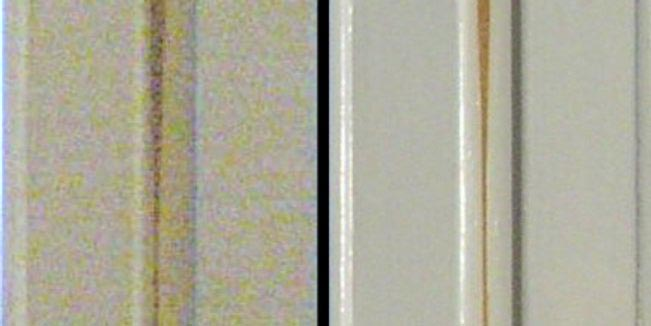
\includegraphics[width=\textwidth]{img/Noise_Comparison}
	\caption{Пример зашумленного изображения.}
	\label{fig:noise_compration}
\end{figure}

Также существуют изображения, полученные не только с фотосенсоров. Примером можно привести рентгенографию, широко используемую во многих областях, таких как медицина, процессы производства и эксплуатации, криминалистика, реставрация и экспертиза художественных ценностей. Существует два варианта получения цифрового изображения рентгенографии, это оцифровка уже существующего рентгеновского снимка, и использование технологии цифровой рентгенографии, при которой сразу идет цифровая обработка получаемого рентгеновского изображения. Оба данных метода подвержены наличию шума на получаемом цифровом изображении, в большей мере шум преобладает на изображених, получаемых первым способом, так как идёт дополнительное наложение шума сканирующим устройством. Пример подобного шума проиллюстрирован на изображении \ref{fig:reng_scan}. Аналогичная ситуация наблюдается и с снимками в области радиографического контроля сварных соединений, пример проиллюстрирован на изображении \ref{fig:reg_met_scan}.

\begin{figure}[h]
	\centering
	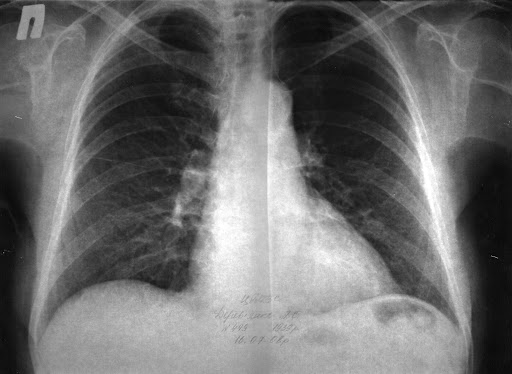
\includegraphics[width=\textwidth]{img/reng_scan}
	\caption{Сканированный рентгеновский снимок грудной клетки человека.}
	\label{fig:reng_scan}
\end{figure}

\begin{figure}[h]
	\centering
	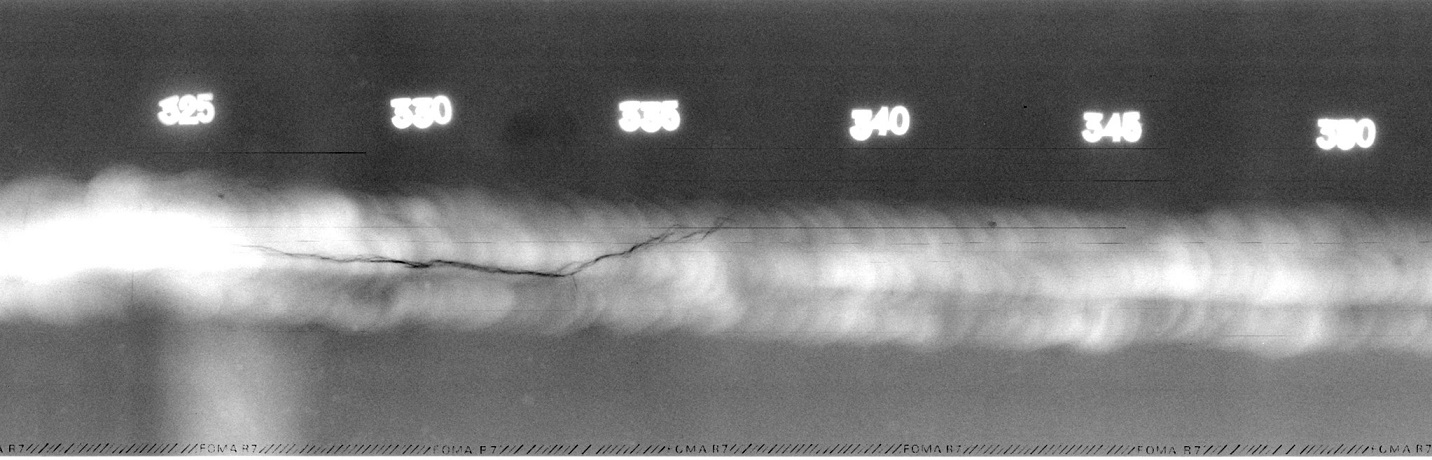
\includegraphics[width=\textwidth]{img/reng_met_scan}
	\caption{Цифровой рентгеновский снимок сварного соединения.}
	\label{fig:reg_met_scan}
\end{figure}

Помимо рентгенографии в обработке медицинских изображений потребность в избавлении полезного сигнала от шума встречаются и в других методах диагностики и визуализации, таких как цифровая реконструкция компьютерной томографии, магнитно-резонансной томографии и других. Потребность в шумоподавлении на медицинских цифровых изображениях изложена в работе~\autocite{MedicalImagesProcessing}.

На данный момент с развитием технологий глубокого обучения и построения глубоких архитектур сверточных нейронных сетей, такие архитектуры применяются к решению широкого ряда задач в области обработки и анализа изображений. Существует три подхода к обучению нейронных сетей: обучение с учителем, обучение без учителя и обучение с подкреплением. Если рассматривать близкие задачи к шумоподавлению с точки зрения построения шаблона обучения сети, это задача увеличения разрешения изображения с помощью нейронных сетей~\autocite{SuperResolutuion:journals/corr/abs-1807-02758} и задача восстановления изображения~\autocite{ImageReconstruction}. Для решения данных задач нейросетевые архитектуры обучаются с помощью подхода обучения с учителем~\autocite{SupervisedLearningReview}. При процессе обучения таких архитектур в качестве входных данных выступают сжатые варианты изображений, подаваемых, как ожидаемые при предсказании сети. Если рассматривать в данном контексте обучение для задачи классификации, то на вход сети необходимо подавать изображение с присутствующем на нём шумом, и обучать сеть предсказывать уже само чистое изображение без шума. 

Все перечисленные способы в этом разделе получения цифрового изображения объединяет один недостаток, это невозможность получения чистого изображения без шума для обучения шумоподавляющей нейронной сети. В данной работе рассматривается подход к построению архитектуры шумоподавляющей нейронной сети и построения обучающего процесса, основанного на методе обучения без учителя (неконтролируемое обучение).

 %Обычно шум на изображении подавляется простыми алгоритмами, к примеру применением медианного фильтра или с помощью гауссова %сглаживания. Также существуют подходы, основанные на использовании нейронных сетей. Но главная проблема их применения заключается в %отсутствие данных для обучения. При обучении шумоподавляющей нейросети в качестве входных данных передаётся зашумленное изображение, а %в качестве ожидаемого ответа необходимо передавать «чистое» входное изображение без шума. В реальных задачах, как правило, нет таких пар %изображений. В данной работе рассматривается задача шумоподалвения цифрового шума.


\chapter{Задача шумоподавления}
\label{sec:init}

\section{Постановка задачи}
Пусть имеется изображение в формате непрерывного сигнала, полученного с АЦП об сигналах матрицы фотосенсора фиксированного цифрового устройства в момент времени $t$ (DNG формат~\autocite{DNG}):
\begin{equation}\label{eq:signal}
S(t)
\end{equation}

Сигнал $S(t)$~(\ref{eq:signal}) состоит из полезного сигнала $G(t)$ и шума $r(t)$, порождаемым фотосенсором:
\begin{equation}\label{eq:signal_decomposition}
S(t)\ =\ G(t)\ +\ r(t)
\end{equation}

При применении преобразования сырого сигнала $S(t)$ к трехмерному дискретному изображению в цветовой схеме RGB получаем матрицу изображения  $\tilde{I}$, с влиянием шума квантования при округлении сигнала при его дискретизации. Подход преобразования $p$ описан в работе Processing RAW Images in MATLAB~\autocite{RAWtoRGB}.
\begin{eqnarray}\label{eq:raw_image_matrix}
\tilde{I}_{i,j} = p(S(t))_{i, j}\ +\ q,\ q  \sim \mathcal{N}(-\frac{1}{2}, \frac{1}{12})\ \text{,}
\end{eqnarray}
где $q$, это шум квантования, семплируемый из нормального распределения с параметрами $\mathcal{N}(-\frac{Q}{2}, \frac{Q}{12})$ при шаге квантования $Q\ =\ 1$, более подробно можно ознакомиться с этим в главе Оценки ошибок (шумов) квантования выходного сигнала в цифровом фильтре из книги Цифровая обработка сигналов~\autocite{DSP}.

Для упрощения постановки задачи будем полагать, что матрица изображения $\tilde{I}$ состоит из суммы изображения, полученного из преобразования чистого (полезного) сигнала $G(t)$~(\ref{eq:signal_decomposition}) в матрицу $I$ и шума $\alpha$, полученного из случайного распределения $\mathbb{P}$, так как появление шума $r(t)$~(\ref{eq:raw_image_matrix})можно считать абсолютно случайным процессом.
\begin{equation}\label{eq:matrix_def}
\tilde{I}\ =\ I\ +\ \alpha,\ \alpha \sim \mathbb{P}
\end{equation}

Таким образом, имея серию из $N$ изображений одной и той же сцены, снятых в разный момент времени $t$ имеем следующую выборку:
\begin{equation}\label{eq:collection}
\{\tilde{I}_k\}_{k=1}^{N}\text{ , где }\tilde{I_k}\ =\  I\ +\ \alpha_k,\ \alpha_k \sim \mathbb{P}
\end{equation}
Причём для каждого элемента из набора $\tilde{I}_k$ компонента $I$ является одним и тем же значением, так как при съёмке одной сцены полезный сигнал $G(t)$~(\ref{eq:signal_decomposition}) остаётся неизменным.

Целью данной работы является построение с помощью нейронной сети приближения отображения $\phi: \mathbb{R}^n \longrightarrow \mathbb{R}^n$, обладающим следующим свойством:
\begin{equation}\label{eq:main_property}
\forall \tilde{I} \in \{\tilde{I}_k\}_{k=1}^{N} \Longrightarrow \phi(\tilde{I}) = I 
\end{equation}
Для построения приближения отображения $\phi$, нейронная сеть $f$ будет обучаться решать следующую задачу оптимизации:
\begin{eqnarray}\label{eq:main_min_task}
\min_{\mathnormal{w}} \Arrowvert f(\tilde{I}, \mathnormal{w}) - I \Arrowvert_{L_2}\text{ ,}
\end{eqnarray}
где $\mathnormal{w}$ - параметры сети $f$, $L_2$ - евклидова норма~\autocite{Haykin}.


\section{Анализируемые данные}
\subsection{Сбор данных}
Так как в данной работе поставлена задача подавления шума у сигнала с заданного сенсора, то изображения для проведения исследования были получены с помощью фиксированного устройства, \textit{Apple iPhone X}, имеющего камеру, состоящую из двух сенсоров.

\begin{table}[h!]
	\centering
	\caption{\label{tab:cam1}Характеристики первого сенсора}
	\begin{tabular}{llr}
		\toprule
		Характеристика  & Значение    & Единица измерения \\
		\midrule
		Разрешение & 12    & $MP$  \\
		Апертура & f/1.8 & \\
		Фокусное расстояние & 28 & $mm$ \\
		Размер сенсора & 1/3" & \\
		Размер пикселя & 1.22 & $\mu m$ \\
		Стабилизация изображения & OIS & \\
		\bottomrule
	\end{tabular}
\end{table}

\begin{table}[h!]
	\centering
	\caption{\label{tab:cam2}Характеристики второго сенсора}
	\begin{tabular}{llr}
		\toprule
		Характеристика  & Значение    & Единица измерения \\
		\midrule
		Разрешение & 12    & $MP$  \\
		Апертура & f/2.4 & \\
		Фокусное расстояние & 52 & $mm$ \\
		Размер сенсора & 1/3.4" & \\
		Размер пикселя & 1.0 & $\mu m$ \\
		Стабилизация изображения & OIS & \\
		\bottomrule
	\end{tabular}
\end{table}

С данного устройства были сделаны серии изображений семи сцен с различным освещением и цветовым наполнением. Данные серии получены стандартными средствами для съёмки на устройстве. При такой съемке автоматически применяются алгоритмы улучшения кадра на устройстве, в том числе и подавление шума. Данные алгоритмы являются коммерческой тайной компании Apple~\autocite{APPLElink}. Под сценой подразумевается съёмка неизменяемой картины реального мира, получая матрицу~(\ref{eq:matrix_def}). Для этого устройство фиксировалось на штативе в неподвижном состоянии  и запуск процесса съёмки кадра производился  с беспроводного устройства, тем самым получая набор изображений $\{\tilde{I}^q_k\}_{k=1}^{N}$~(\ref{eq:collection}), где $q$ - порядковый номер снимаемой сцены. Для каждой сцены при съемке были зафиксированны значения ISO, фокуса и цветовой температуры. 

% 95 фотографий
Каждая сцена содержит в среднем по $14$ фотографий, суммарное количество кадров из всех наборов составляет $95$ изображений.


Так как стандартные средства для съёмки не позволяют получать RAW (изображение с сырого сигнала АЦП~(\ref{eq:signal})) изображение, то были произведены съёмки дополнительных сцен с использованием стороннего программного обеспечения, позволяющего получать <<сырые>>  кадры в формате TIFF~\autocite{TIFFArticle}: Simple Raw camera~\autocite{RAWCamera}. С помощью данного приложения были сняты серии трёх дополнительных сцен. Данные серии содержат суммарно $30$ изображений, ровно по $10$ кадров в каждой серии.

Максимальное количество изображений в одной серии ограничено $20$-ю кадрами, так как при продолжении процесса съёмки фотосенсор нагревается и из-за теплового воздействия появляются дополнительные искажения сигнала, из-за которых теряется попиксельное соответствие кадров в серии между собой.

В итоге получается набор данных, состоящий из $125$ изображений, снятых на один сенсор. Визуальное различие шума на изображениях, полученных разными подходами можно рассмотреть на рисунке~\ref{fig:noise_comprasion}.

Также для сравнения результатов были сделаны 6 серий, снятых следующей web камерой~\autocite{WebCam} в разрешении $1920\times1080$. Снимались видеозаписи короткой длительности и разбивались на кадры с помощью библиотеки FFmpeg~\autocite{FFMPEG}. Суммарное количество кадров в данных сериях составило $811$.

\begin{figure}[h]
	\centering
	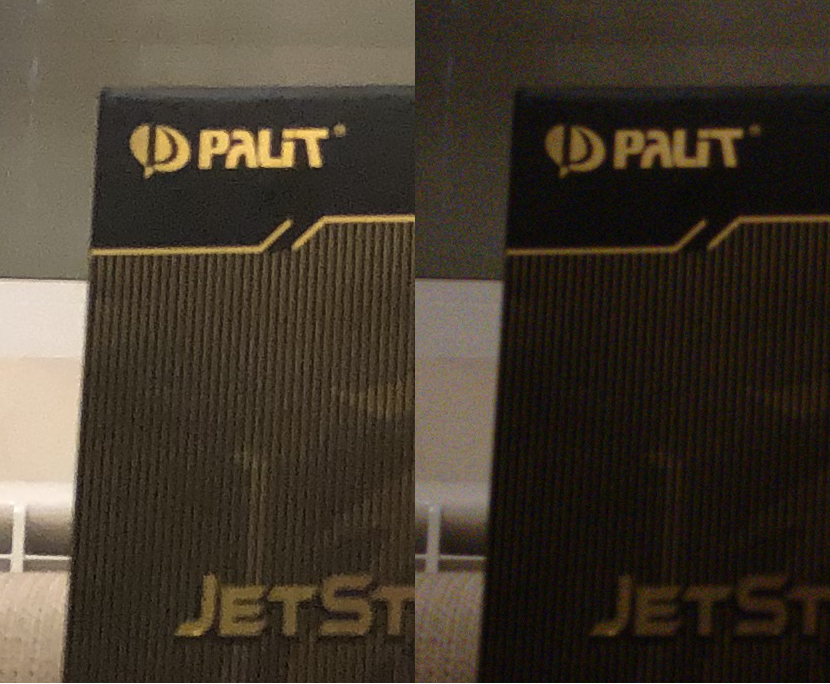
\includegraphics[width=\textwidth]{img/noise_comprasion}
	\caption{Сравнение получаемого шума на изображении, снятого стандартными средствами устройства (слева) и RAW изображения (справа)}
	\label{fig:noise_comprasion}
\end{figure}


\subsection{Анализ собранных данных}

Во время процесса съемки при нагреве фотосенсора могут происходить незначительные искажения кадра. Или также возможны незаметные смещения устройства при съемке, а также смена внешних условий, таких как освещение или движение объектов в кадре. Для собираемого набора изображений сдвиг более чем на один пиксель между кадрами одной серии уже критичен.

Для анализа качества полученных серий изображений были построены распределения $e^q$~(\ref{eq:series_distribution}) отклонений каждого изображения от усредненного по всем изображениям из серии $\hat{I}^q$~(\ref{eq:mean_image}) по евклидовой метрике.
\begin{eqnarray}\label{eq:mean_image}
\hat{I}^q_{i,j}\ =\ \sum_{k}\tilde{I}^q_{k\ i,j}
\end{eqnarray}

\begin{eqnarray}\label{eq:series_distribution}
e^q_k\ =\ \Arrowvert \hat{I}^q - \tilde{I}^q_k \Arrowvert_{L_2}
\end{eqnarray}
Дополнительно производится нормировка выборки по метрике $L_1$:
$$e^q_k\ =\ \frac{e^q_k}{\sum_{i}(e^q_i)}$$

Далее по значениям выборки $e^q$~(\ref{eq:series_distribution}) строятся графики плотности нормального распределения $\mathcal{N}(\mu, \sigma)$ с параметрами:
\begin{eqnarray}\label{eq:mean_and_std}
\mu^q = \mu(e^q),\ \sigma^q = \sigma(e^q)
\end{eqnarray}

Таким образом математическое ожидание $\mu^q$~(\ref{eq:mean_and_std}) показывает насколько усредненное изображение $\hat{I}^q$~(\ref{eq:mean_image}) близко к изображению, теоретически, получаемому из чистого сигнала $I^q$~(\ref{eq:collection}): 
$$\hat{I}^q \xrightarrow[\mu^q \rightarrow 0]{} I^q$$
А также, чем ближе к $0$ значение среднеквадратичного отклонения выборки $\sigma^q$~(\ref{eq:mean_and_std}), тем на большем количестве изображений из серии присутствует сигнал $G(t)$~(\ref{eq:signal_decomposition}), зафиксированный в момент времени $t = t_0$, то есть насколько сцена неизменна между кадрами.

Графики распределений для серий, снятых стандартными средствами устройства \textit{Apple iPhone X} изображен на рисунке~\ref{fig:distribuion_after_apple_denoising}. Из графиков можно увидеть, что чем больше размер серии, тем ближе усредненное изображение к чистому.

\begin{figure}[h!]
	\centering
	\includegraphics[width=\textwidth]{img/series_apple_denoising_deviation_comparison}
	\caption{Графики плотностей нормальных распределений для серий, снятых стандартными средствами устройства \textit{Apple iPhone X}}
	\label{fig:distribuion_after_apple_denoising}
\end{figure}


Рассматриваемый параметр $\sigma$~(\ref{eq:mean_and_std}) сильно зависит не только от движения объектов на снимаемой сцене, но и от уровня освещения. Сдвиг объектив особо критичен, так как обученная нейросеть на такой выборке будет размывать результирующие изображение. Сравнение усредненного изображения, имеющего сдвиг сцены с изображением, полученным из усреднения кадров статичной сцены изображено на рисунке~\ref{fig:deviations_comparision}. 

\begin{figure}[H]
	\centering
	\includegraphics[width=\textwidth]{img/incorrect_and_correct_comparison}
	\caption{Для среднего изображения серии слева $\sigma = 0.00891$, для среднего изображения серии справа $\sigma = 0.00272$}
	\label{fig:deviations_comparision}
\end{figure}

Также большое значение отклонения $\sigma$~(\ref{eq:mean_and_std}), полученное из-за сильного изменения освещения при съемке также неблагоприятно скажется на качестве обучения нейронной сети, так как нейронная сеть, обученная на таких сериях, не сможет корректно предсказывать цветовую гамму результирующего изображения. Пример зависимости параметра отклонения от уровня освещения снимаемой сцены при естественном освещении изображен на рисунке~\ref{fig:hists_comparision}. Из данного примера  можно заметить, что незначительные отклонения в освещении, различимые по небольшим отличиям в цветовых гистограммах изображений из серии сильно влияют на параметр $\sigma$~(\ref{eq:mean_and_std}), и для данной статичной сцены данный параметр близок к значению, получаемому у сцены с сильным сдвигом~\ref{fig:deviations_comparision}.


\begin{figure}[H]
	\centering
	\includegraphics[width=\textwidth]{img/imgs_8_series_stack_image}
	\caption{Серия изображений с цветовыми гистограммами, параметр $\sigma$ данной серии равен $0.00608$ }
	\label{fig:hists_comparision}
\end{figure}

Для остальных условий съемки аналогичным образом были построены графики с распределениями, изображенные на рисунках~\ref{fig:distribuion_real_noise},~\ref{fig:distribuion_real_noise_good_condition} и~\ref{fig:distribuion_webcam}. Серии, полученные с web камеры содержат относительно большое количество кадров каждой сцены (в среднем по $135$) и не подвергаются искажениям из-за нагрева сенсора за счет большего шага дискретизации изображения реального мира (меньшего разрешения).

\begin{figure}[H]
	\centering
	\includegraphics[width=\textwidth]{img/night_condition_series_real_noise_iphone_deviation_comparison}
	\caption{Графики плотностей нормальных распределений для серий, снятых при условиях плохого искусственного освещения с помощью приложения~\autocite{RAWCamera}}
	\label{fig:distribuion_real_noise}
\end{figure}


\begin{figure}[H]
	\centering
	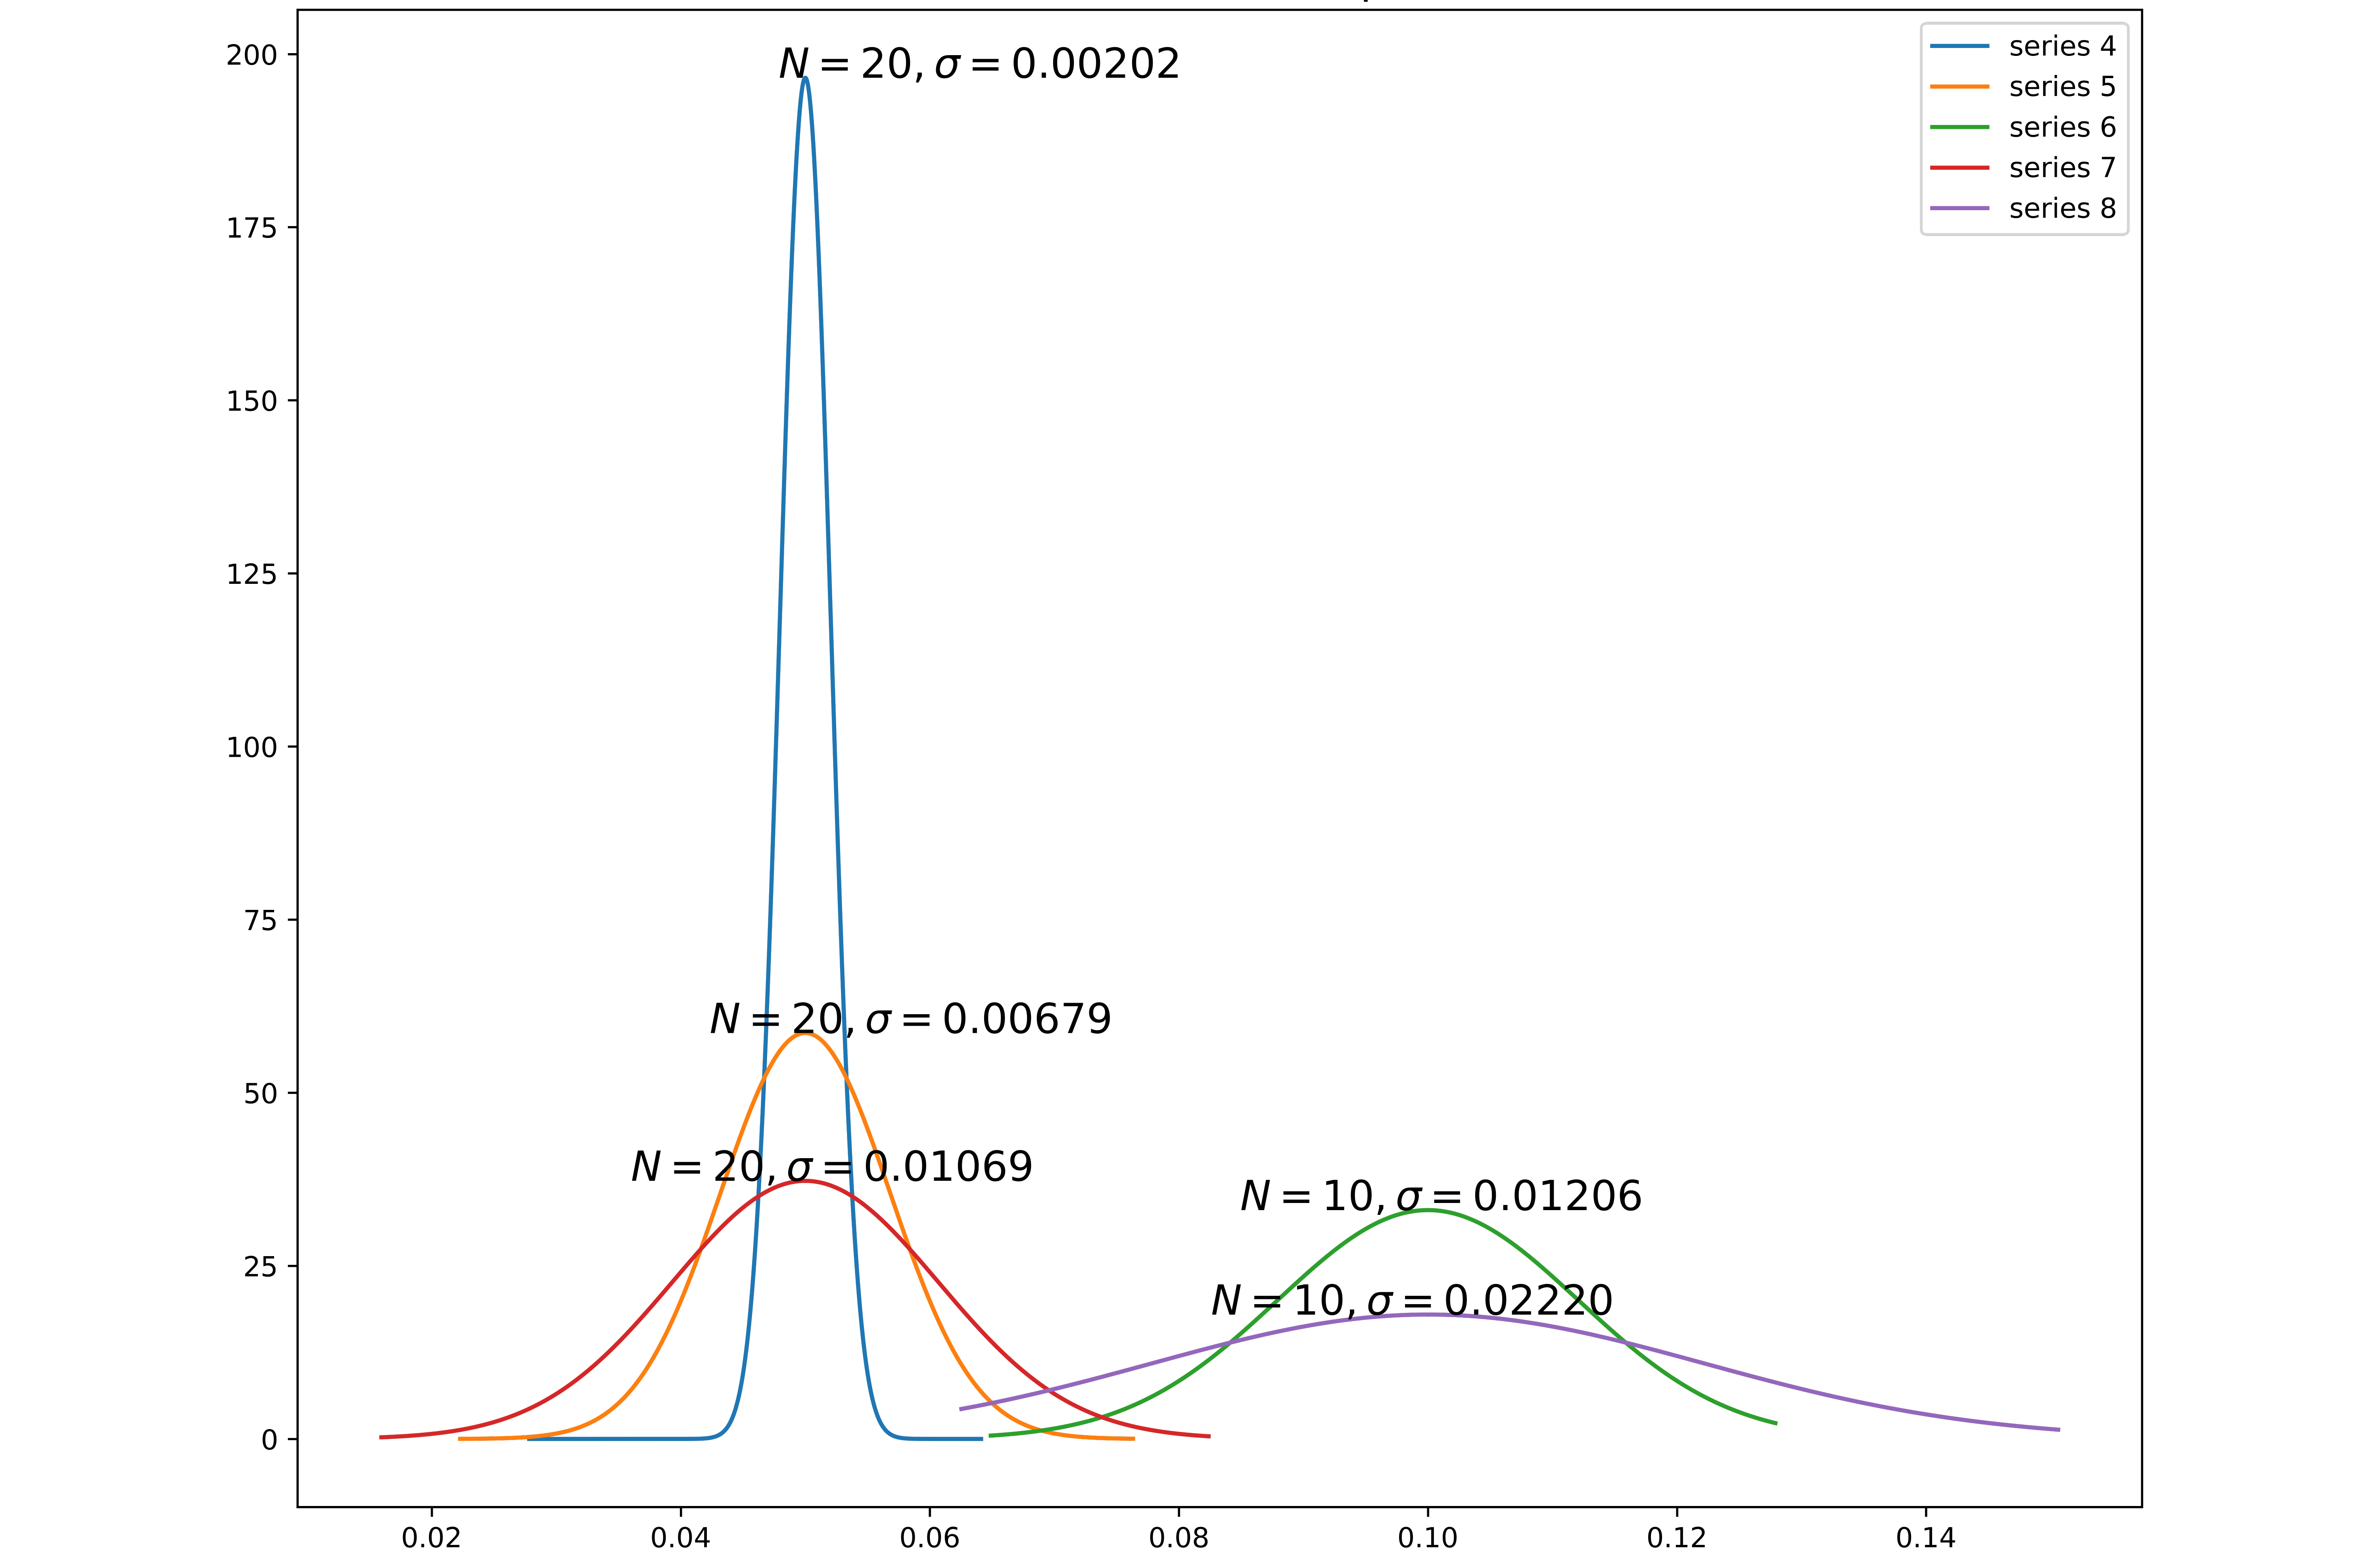
\includegraphics[width=\textwidth]{img/good_condition_series_real_noise_iphone_deviation_comparison}
	\caption{Графики плотностей нормальных распределений для серий, снятых при условиях естественного освещения с помощью приложения~\autocite{RAWCamera}}
	\label{fig:distribuion_real_noise_good_condition}
\end{figure}

\begin{figure}[H]
	\centering
	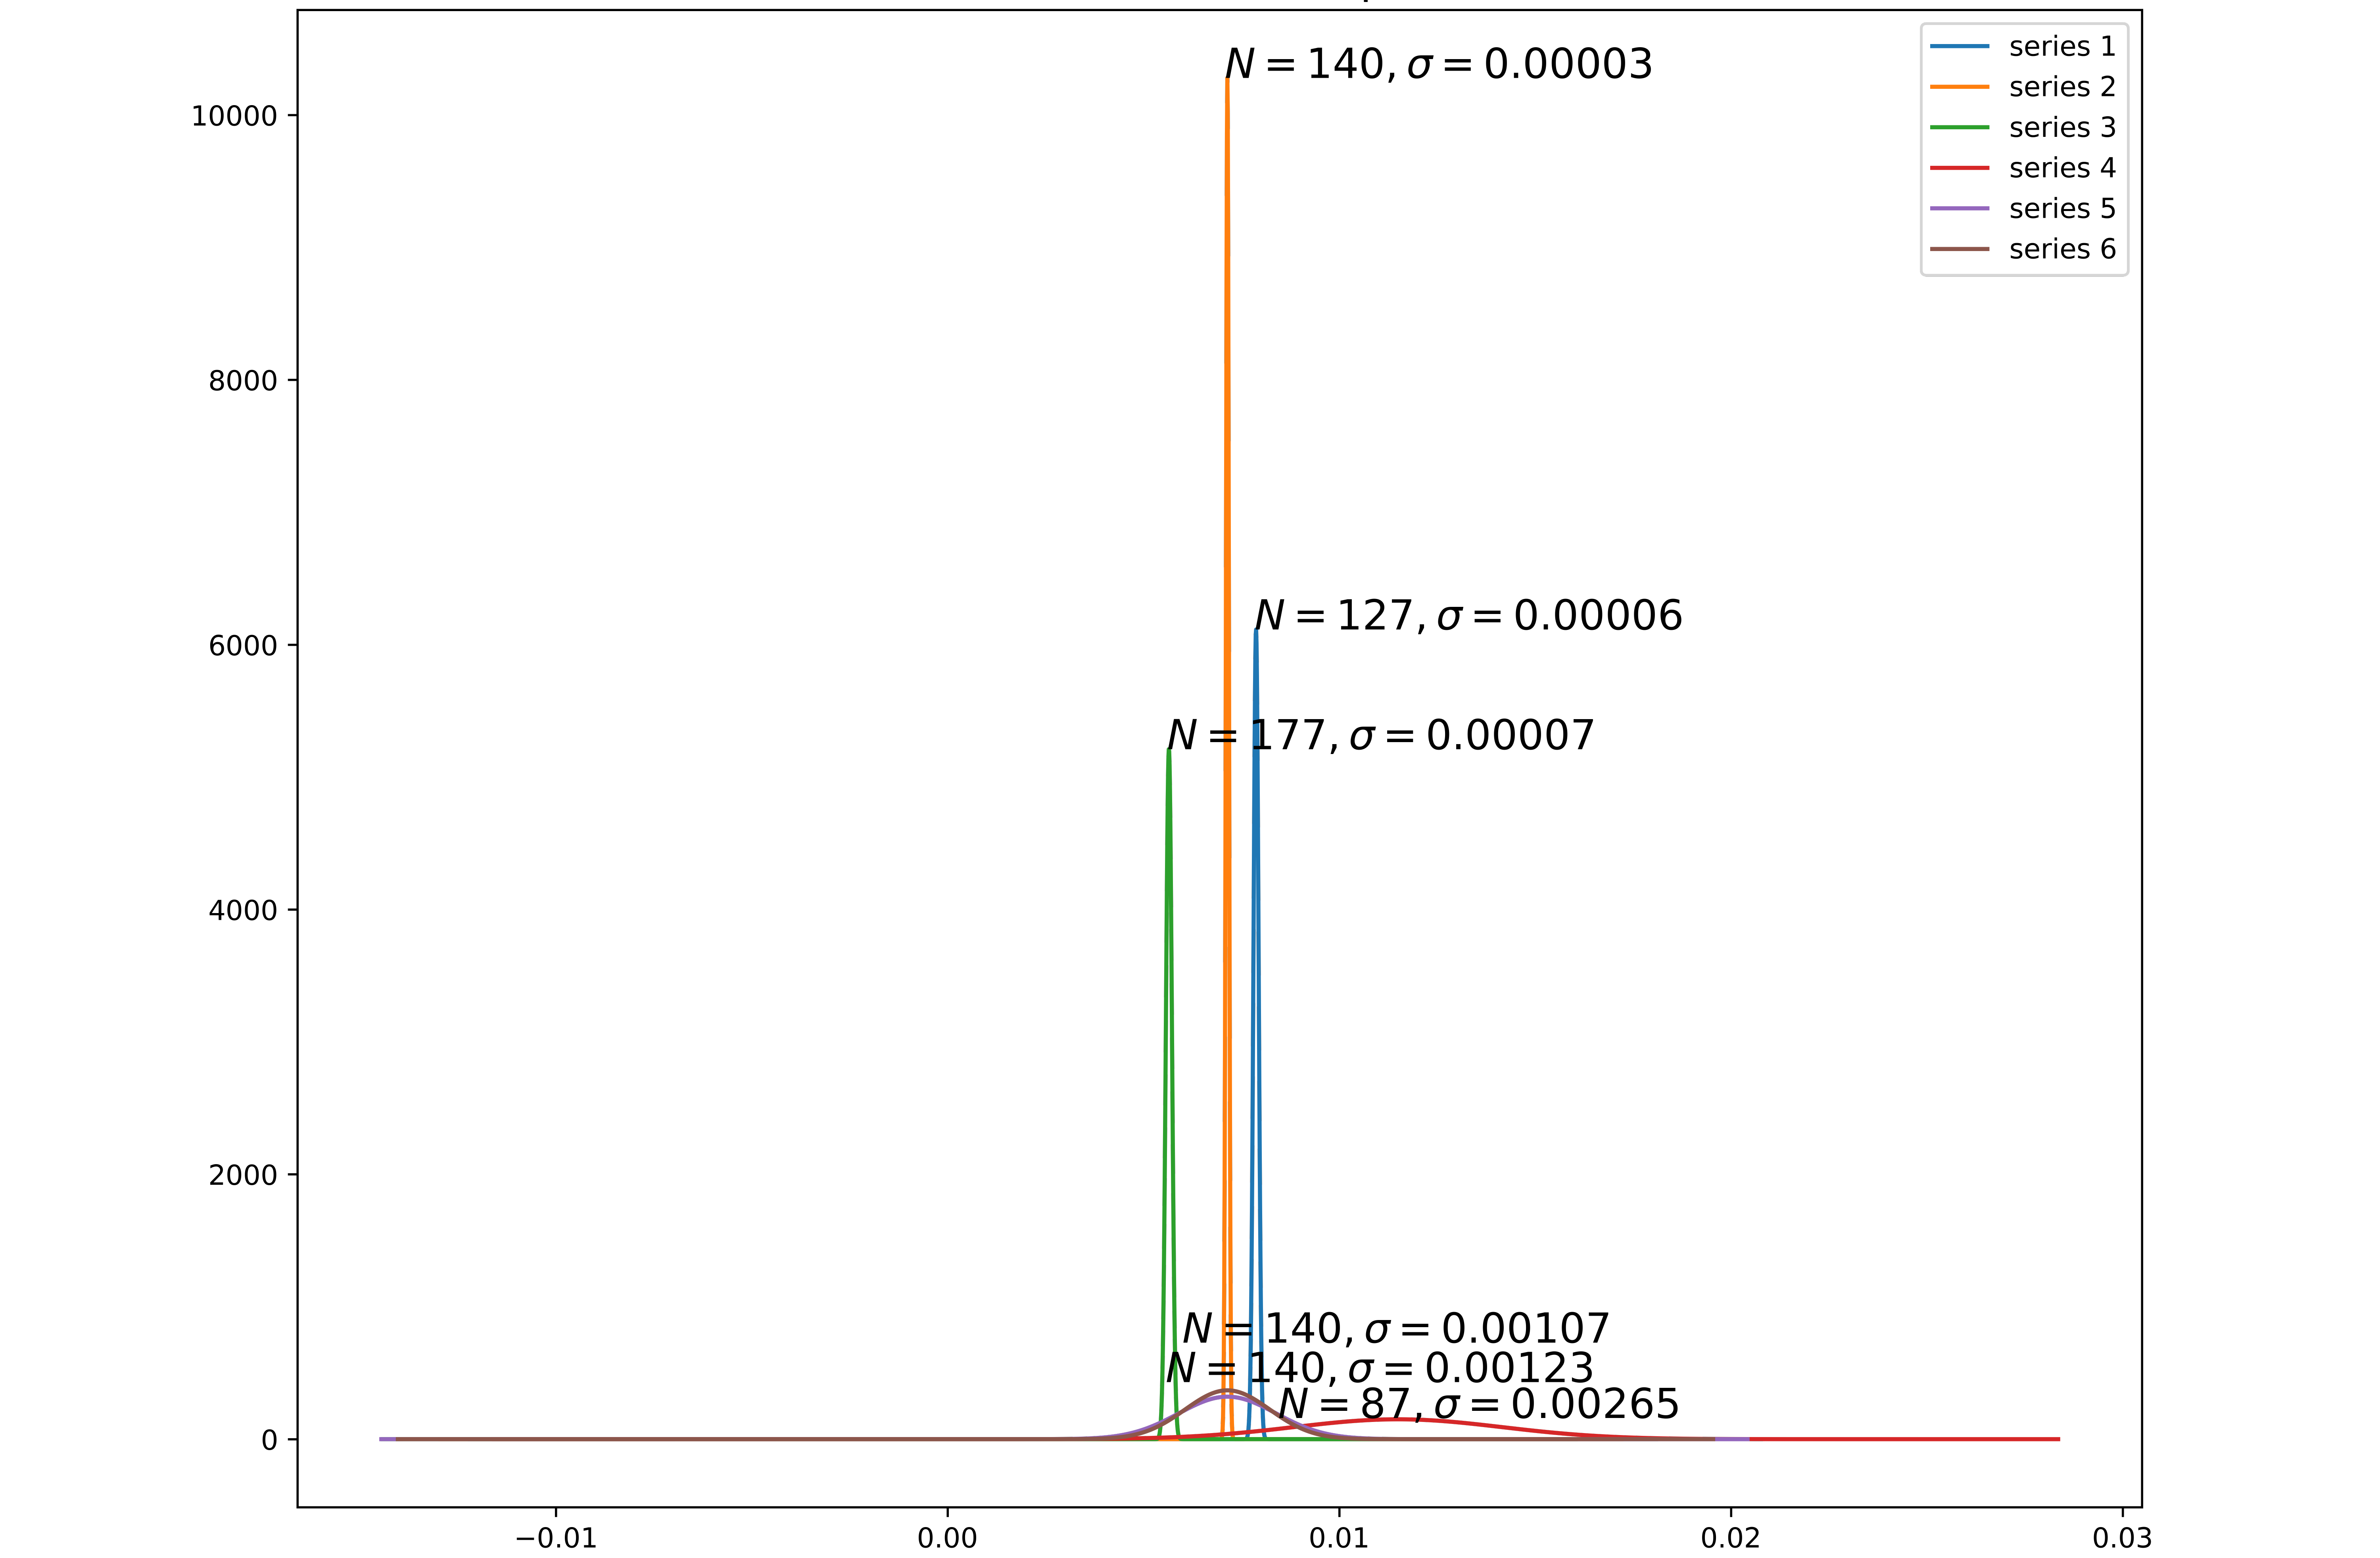
\includegraphics[width=\textwidth]{img/series_webcam_deviation_comparison}
	\caption{Графики плотностей нормальных распределений для серий, снятых при разных условиях освещения с помощью web камеры~\autocite{WebCam}}
	\label{fig:distribuion_webcam}
\end{figure}


При выборе данных для обучения нейронных сетей подавляющих шум на изображении задается условие, что параметр $\sigma$~(\ref{eq:mean_and_std}) не должен превышать значения $0.007$

\section{Существующие решения}
\subsection{Подходы, не использующие нейронные сети}

\subsubsection{Гауссовское размытие}
Одним из самых распространённых подходов подавления шума на изображении является применение гауссовского размытия. Оно заключается в свертке изображения с ядром, полученным следующей функцией:
\begin{eqnarray}\label{eq:gauss_kernel_function}
g(x, y)\ =\ A e^{-\frac{x^2 + y^2}{\sigma^2}}
\end{eqnarray}
где параметр $\sigma$ задаёт степень размытия, а параметр $A$ обеспечивает нормировку. Более детально данный подход описан в работе~\autocite{GaussianBilinear}.

Основным достоинством данного подхода является простота реализации алгоритма и быстрая скорость работы. Также данный подход имеет реализацию во всех популярных библиотеках для обработки изображений на языках программирования Python и C/C++, таких как OpenCV~\autocite{OpenCVLib}.

Если рассматривать данный подход применительно к анализируемым данным, то подход справляется только с шумом, полученным после обработки стандартными средствами съемки устройства, но и при этом можно заметить размытие кадра уже с использованием свертки размера $5$. Результат можно увидеть на рисунке~\ref{fig:apple_noise_gauss_comparison}. Если рассматривать применительно к сырым RAW изображениям, то и при сильном размытии остается заметный шум и при этом сильно размывается изображением. Результат такого применения можно увидеть на изображении~\ref{fig:real_noise_gauss_comparison}. Для получения данных результатов использовалась реализация из библиотеки OpenCV~\autocite{OpenCVLib}.

\begin{figure}[h]
	\centering
	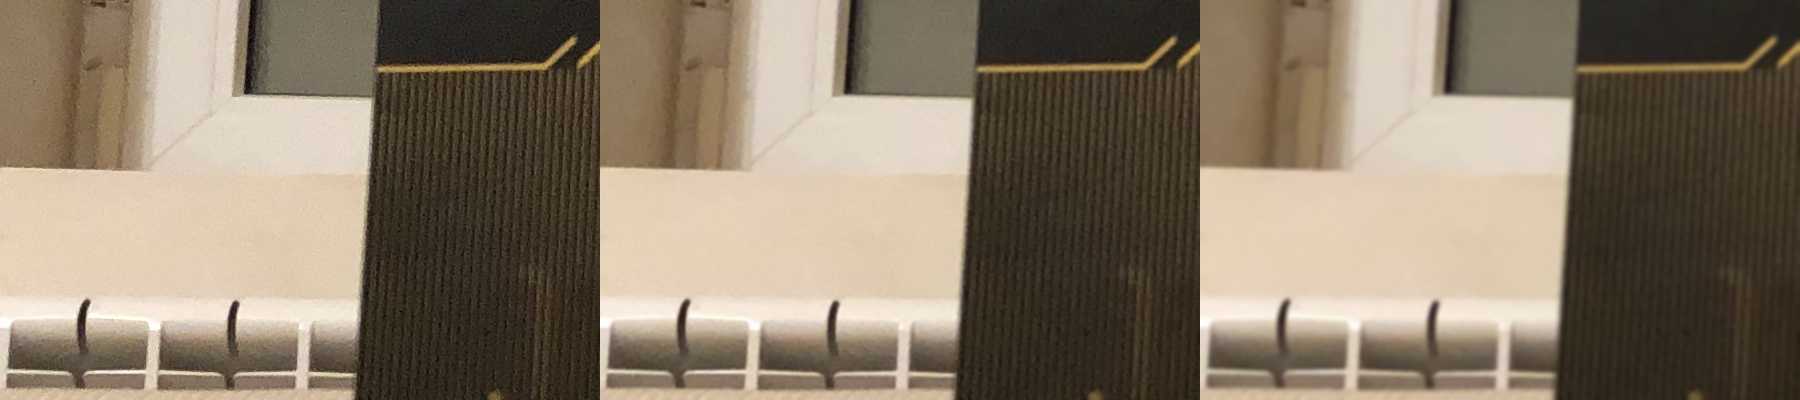
\includegraphics[width=\textwidth]{img/apple_noise_gaussian_params_comparison}
	\caption{Результат работы гауссовского размытия на изображении со стандартной обработкой телефона. Слева направо: оригинальное изображение, с применением размытия с параметром $\sigma = 1$ и размером ядра $5$, с применением размытия с параметром $\sigma = 2$ и размером ядра $9$}
	\label{fig:apple_noise_gauss_comparison}
\end{figure}

\begin{figure}[h]
	\centering
	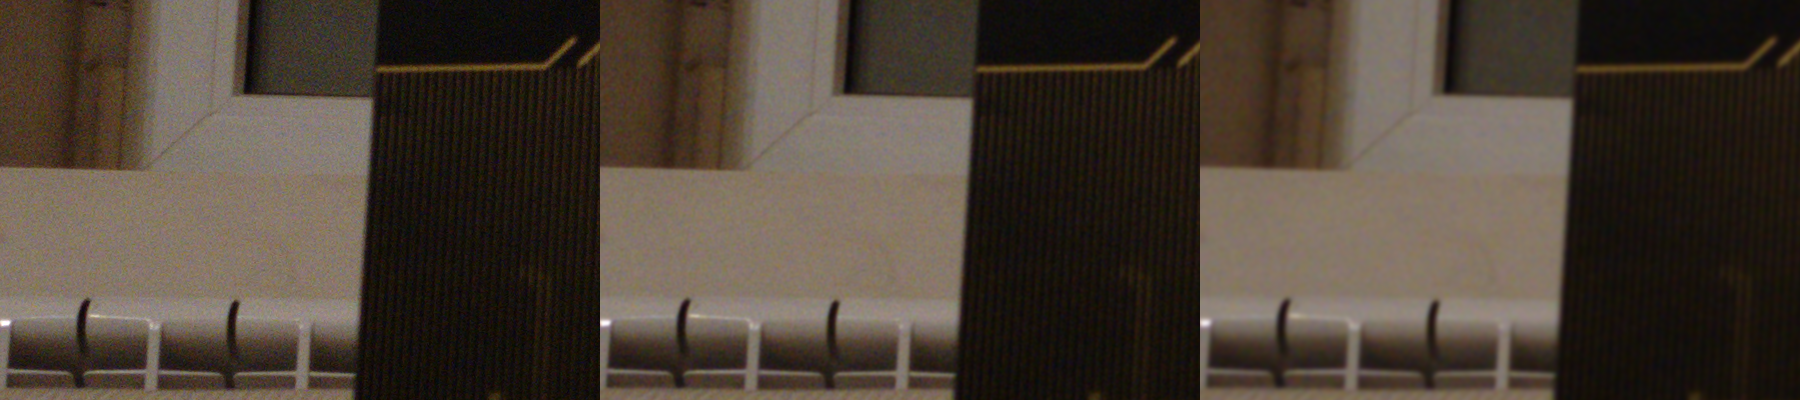
\includegraphics[width=\textwidth]{img/real_noise_gaussian_params_comparison}
	\caption{Результат работы гауссовского размытия на сыром (RAW) изображении. Слева направо: оригинальное изображение, с применением размытия с параметром $\sigma = 1$ и размером ядра $5$, с применением размытия с параметром $\sigma = 2$ и размером ядра $9$}
	\label{fig:real_noise_gauss_comparison}
\end{figure}

\subsubsection{Медианный фильтр}

Медианный фильтр реализуется следующим образом: для каждого пикселя в некотором окружении окна, заданного размера $d,\ d\ mod\ 2 == 1$ находится медианное значение данного набора пикселей и присваивается текущему. Также индекс медианного пикселя для рассматриваемого пикселя $p$ можно представить в следующем виде:
\begin{equation}
median\ index\ =\ \arg\ \min_{p_i \in P} \sum_{p_j \in P} \Arrowvert p_i - p_j \Arrowvert_{L_1}
\end{equation}
$$P = \{I_{i, j}\}_ {(i - i_p)^2 + (j - j_p)^2 \le d^2},\ \text{где }i_p, j_p\text{ координаты пикселя }p$$

Результат применения реализации данного метода из библиотеки OpenCV~\autocite{OpenCVLib} на анализируемых данных изображен на рисунке~\ref{fig:medianblur_comparison}. Эффекта подавления шума на обоих примерах удается при значении параметра $d = 15$, но при этом изображения имеют потерю высоких частот. Подробно данный метод описан в работе~\autocite{MedicalImagesProcessing}. 

\begin{figure}[h]
	\centering
	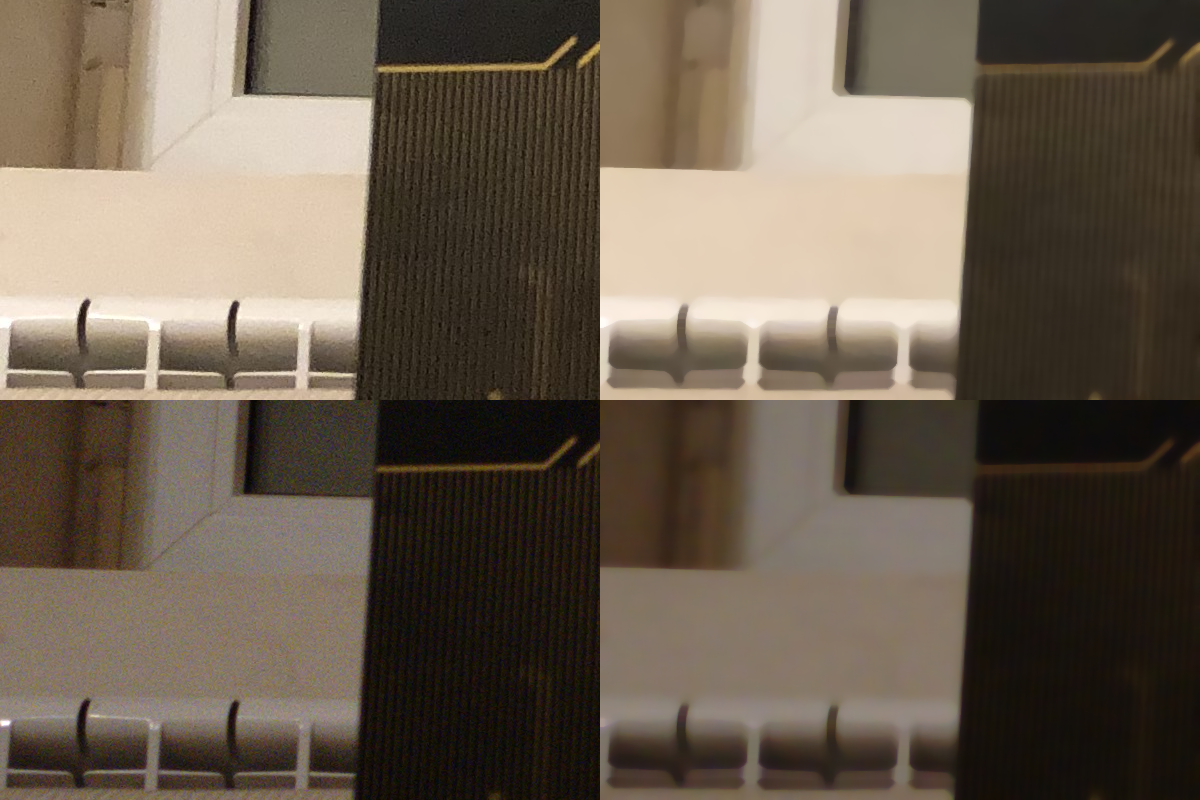
\includegraphics[width=\textwidth]{img/medianfilter_comparison}
	\caption{Применение медианного фильтра для обработанного стандартными средствами изображения (сверху) и чистого RAW изображения (снизу)}
	\label{fig:medianblur_comparison}
\end{figure}

\subsubsection{Двустороннее сглаживание}
Двусторонняя фильтрация (Bilateral filtering) сглаживает изображения при сохранении краев посредством нелинейной комбинации соседних значений изображения. Данный подход описан в работе~\autocite{BilateralPaper}. Данный метод подавления шума, как и предыдущие является широко распространенным и имеет реализации в большинстве библиотек для работы с изображениями. 

Применяя данный алгоритм к анализируемым данным, можно увидеть, что он хорошо справляется с шумом, содержащимся в сырых RAW изображениях, но при этом теряются высокие частоты изображения, что приводит к размытию линий в нижней левой части кадра из примера, изображенного на рисунке~\ref{fig:bilinear_comparison}. Применение данного алгоритма к предобработанным стандартными средствами устройства изображениям не дает ощутимого результата, это можно увидеть на изображении~\ref{fig:bilinear_comparison}. В обоих случаях использовалась реализация из библиотеки OpenCV~\autocite{OpenCVLib} с параметром радиуса $r = 15$.

\begin{figure}[h]
	\centering
	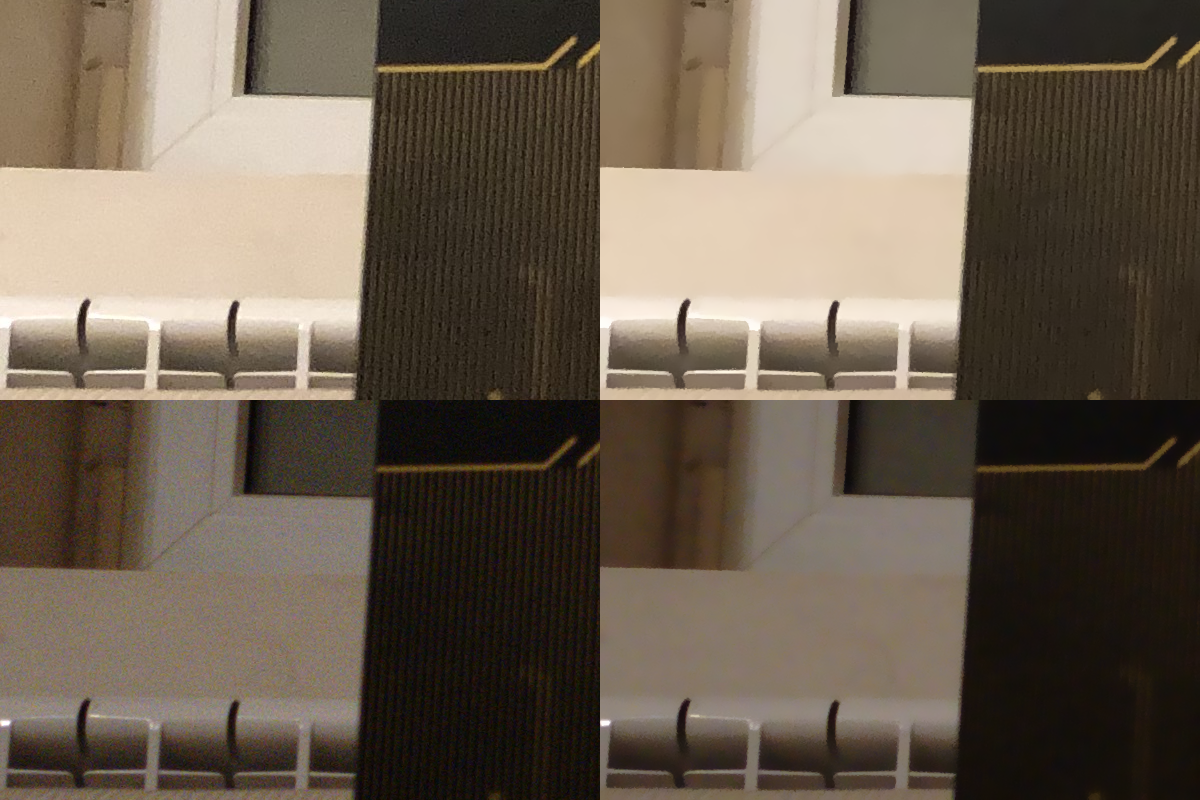
\includegraphics[width=\textwidth]{img/bilinear_comparison}
	\caption{Применение метода двусторонней фильтрации для обработанного стандартными средствами изображения (сверху) и чистого RAW изображения (снизу)}
	\label{fig:bilinear_comparison}
\end{figure}

\subsubsection{Non-Local Means Denoising}

\subsection{Подходы, основанные на нейросетях}

% Печать списка литературы (библиографии)
\printbibliography[%{}
    heading=bibintoc%
    %,title=Библиография % если хочется это слово
]
% Файл со списком литературы: biblio.bib
% Подробно по оформлению библиографии:
% см. документацию к пакету biblatex-gost
% http://ctan.mirrorcatalogs.com/macros/latex/exptl/biblatex-contrib/biblatex-gost/doc/biblatex-gost.pdf
% и огромное количество примеров там же:
% http://mirror.macomnet.net/pub/CTAN/macros/latex/contrib/biblatex-contrib/biblatex-gost/doc/biblatex-gost-examples.pdf

\end{document}
